\section{Computational study}\label{sec:computation}

All timings are wall-clock on a 28-core workstation, with no other experiment running, to a relative optimality gap of $5\cdot10^{-4}$.
Scenarios are drawn from the true demand distribution of a regular day unless stated otherwise.

\paragraph{Extensive form vs.\ decomposition.}
\begin{table}[t]
\centering\small
\caption{Extensive form (HiGHS MIP, 1800\,s limit) vs.\ Benders (\cref{alg:benders}) with 1 and 24 subproblem workers. Speed-up: extensive form vs.\ Benders with 24 workers.}\label{tab:scaling}
\begin{tabular}{@{}rrrrrrrrr@{}}\toprule
 & \multicolumn{3}{c}{Extensive form (HiGHS MIP)} & \multicolumn{4}{c}{Benders} & Speed-up \\
\cmidrule(lr){2-4}\cmidrule(lr){5-8}
$N$ & columns & time (s) & gap (\%) & 1 worker (s) & 24 workers (s) & gap (\%) & iter. & \\ \midrule
5 & 12{,}805 & 3 & 0.008 & 14.9 & 15.0 & 0.050 & 45 & 0.2$\times$ \\
10 & 25{,}480 & 6 & 0.016 & 4.0 & 9.7 & 0.041 & 33 & 0.6$\times$ \\
25 & 63{,}505 & 23 & 0.015 & 7.0 & 4.0 & 0.048 & 20 & 5.7$\times$ \\
50 & 126{,}880 & 48 & 0.042 & 24.2 & 16.6 & 0.028 & 18 & 2.9$\times$ \\
100 & 253{,}630 & 174 & 0.037 & 43.2 & 14.6 & 0.039 & 17 & 12$\times$ \\
\bottomrule\end{tabular}

\end{table}

\Cref{tab:scaling} compares the deterministic equivalent solved directly by HiGHS with the decomposition.
HiGHS is a strong MIP solver and handles the extensive form well for few scenarios: at $N=5$ it is five times faster than Benders.
Its solve time grows superlinearly with the number of scenarios, however: 47\,s at $N=50$ and 174\,s at $N=100$, with 254{,}000 columns.
Benders' solve time, in contrast, barely moves.
The decomposition wins from $N=10$ with one worker and from $N=25$ with 24 workers, where pool overhead is amortised. At $N=100$ it is $12\times$ faster with 24 workers ($4\times$ with one).

\begin{figure}[t]
  \centering
  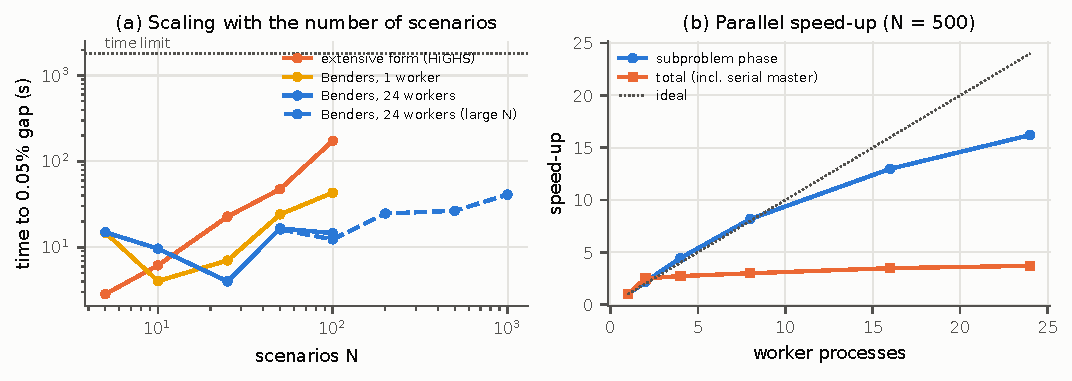
\includegraphics[width=\linewidth]{scaling}
  \caption{(a) Time to a 0.05\% gap as a function of the number of scenarios. (b) Parallel speed-up for $N=500$: the subproblem phase scales well, the total is limited by the serial master problem (Amdahl's law).}
  \label{fig:scaling}
\end{figure}

\paragraph{Scaling to many scenarios and parallelism.}
With 24 workers, Benders solves $N=1000$ (2.5 million recourse columns) in 41\,s (\cref{fig:scaling}a).
The number of iterations is essentially independent of $N$ (16--18).
The phase-1 Jensen block gives the master a scenario-independent description of the capacity structure, and multi-cut lets every scenario contribute its own cut in each iteration.
Parallel subproblems scale well: the subproblem phase at $N=500$ is $16\times$ faster with 24 workers than with one (\cref{fig:scaling}b).
The total speed-up, however, is only $3.7\times$, because the master MIP is solved serially and accounts for over 90\% of the time with many workers.
The natural next step is therefore not more workers but a single-tree \emph{branch-and-Benders-cut}, in which cuts are added as lazy constraints inside one branch-and-bound search instead of re-solving the master MIP in every iteration.

\paragraph{Ablation.}
\begin{table}[t]
\centering\small
\caption{Ablation of the Benders components ($N=50$, 24 workers, three regular test days, 900\,s limit). Each row adds one component to the row above, up to ``+Jensen (phase 1)'', which is the configuration used everywhere else. The last three rows are variations of it. Master: share of the time spent in the master problem. $^\dagger$Time limit reached on at least one day.}\label{tab:ablation}
\resizebox{\linewidth}{!}{\begin{tabular}{@{}lrrrrrrr@{}}\toprule
Variant & mean time (s) & max time (s) & iterations & LP iter. & cuts & max gap (\%) & master (\%) \\ \midrule
classic$^\dagger$ & 927.0 & 963.7 & 95 & 0 & 4750 & 0.076 & 100 \\
+LP phase & 53.5 & 90.5 & 88 & 86 & 4416 & 0.045 & 97 \\
+in-out & 38.2 & 47.6 & 52 & 49 & 2616 & 0.037 & 97 \\
+Jensen (phase 1) & 9.9 & 11.9 & 18 & 15 & 882 & 0.042 & 96 \\
+Jensen (both phases) & 10.7 & 22.9 & 18 & 15 & 882 & 0.039 & 96 \\
+Jensen x4 (phase 1) & 7.6 & 12.3 & 13 & 10 & 633 & 0.042 & 96 \\
single-cut (all)$^\dagger$ & 905.3 & 908.6 & 346 & 150 & 346 & 0.113 & 99 \\
\bottomrule\end{tabular}
}
\end{table}

\begin{figure}[t]
  \centering
  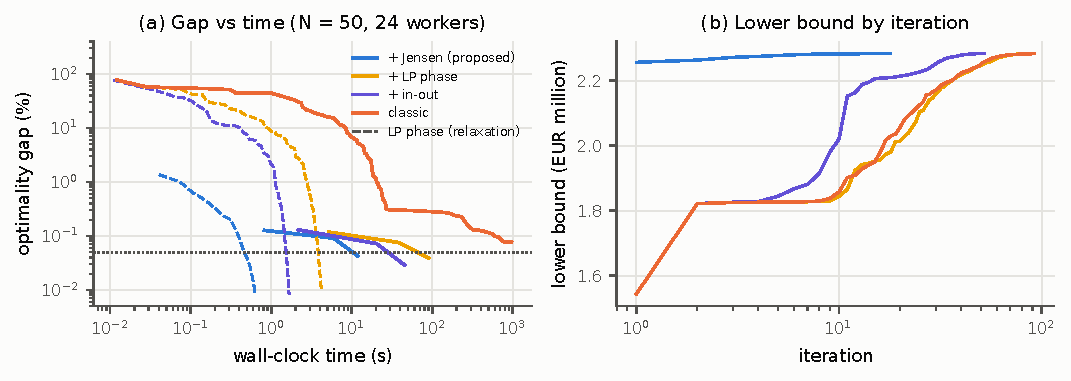
\includegraphics[width=\linewidth]{convergence}
  \caption{Convergence of the ablation variants on 5 March 2026. (a) Optimality gap against time. Dashed: gap of the LP relaxation during the LP phase; solid: true gap of the integer problem (best integer solution vs.\ best bound). Dotted line: the 0.05\% target. (b) Lower bound by iteration; the Jensen block makes the first bound almost tight.}
  \label{fig:convergence}
\end{figure}

\Cref{tab:ablation,fig:convergence} isolate the contribution of each component.
\begin{itemize}
  \item \textbf{Classic multi-cut Benders} reaches the 0.05\% target on only one of the three days within 900\,s. In its first ten iterations the cuts carry almost no information about the capacity structure and the lower bound stays flat (\cref{fig:convergence}b).
  \item \textbf{The LP phase} is the largest single gain: it generates most cuts from cheap master LPs, and the time falls to 54\,s on average.
  \item \textbf{In-out stabilisation} reduces the number of iterations by 40\% and the mean time to 38\,s. It is not uniformly better: on one of the three days it is slower than the LP phase alone (48\,s vs.\ 33\,s).
  \item \textbf{The Jensen block} gives the master a valid, scenario-independent approximation of the recourse from the first iteration. The first lower bound is within 1.2\% of the optimum, the iterations drop to 18 and the time to 10\,s. In total the method is at least $90\times$ faster than classic Benders; ``at least'' because classic Benders hit the time limit on two days.
  \item \textbf{Variations.} Keeping the Jensen block in the integer phase does not help on average and is slower on one day (23\,s): it adds rows to every master MIP. Four Jensen blocks instead of one save another 25\% (7.6\,s). We keep the simpler single block.
  \item \textbf{Single-cut} Benders (one aggregated cut per iteration) does not reach the target in 900\,s even with all other components: aggregating 50 scenarios into one cut throws away most of the information returned by the subproblems.
\end{itemize}
In every variant the master accounts for 96--100\% of the time. The subproblems, warm-started and solved in parallel, are not the bottleneck; this again points to branch-and-Benders-cut as the next step.

\paragraph{Larger networks.}
All results above are for the Iberian network (130 integer variables). On a synthetic network of the same size (10 FCs, 12 SCs, 65 zones, $N=50$), Benders behaves as on the real one: 26\,s and 22 iterations. On a synthetic network twice as large (20 FCs, 25 SCs, 150 zones, 520 integer variables), it did not reach the 0.05\% target within an hour, and we stopped the experiment. Since the subproblems are not the bottleneck, this is the serial master MIP again: scaling to national networks with hundreds of sites needs branch-and-Benders-cut, or a master that is itself decomposed by region. We list this as the main computational limitation (\cref{sec:discussion}).

